\documentclass[10pt,a4paper]{article}
\usepackage[utf8]{inputenc}
\usepackage{amsmath}
\usepackage{amsfonts}
\usepackage{graphicx}
\usepackage{amssymb}
\usepackage[hidelinks]{hyperref}
\hypersetup{
    colorlinks,
    citecolor=black,
    filecolor=black,
    linkcolor=black,
    urlcolor=black
}
\usepackage{amsmath}
\DeclareMathOperator*{\argmax}{arg\,max}
\DeclareMathOperator*{\argmin}{arg\,min}
\author{Louis Cohen}
\title{Steiner Tree Problem Optimization}
\begin{document}

\maketitle	

\tableofcontents

\section{Abstract}

Dans ce rapport je presenterai différentes approches choisies pour approximer le probleme des arbres de Steiner. Basé sur le papier ref ref pour les choix des voisins. 

\section{Introduction}

Le problème des arbres de Steiner est un problème de graphe NP Complet. Il consiste à, pour un graphe pondéré et un sous ensemble de noeuds (les terminaux), trouver le sous ensemble d'aretes de poids minimal connectant ces terminaux. Ce problème largement étudié trouve de nombreuses applications blablabla. Il n'est évidemmnet pas possible de résoudre completement le problème dans le cas général. Cependant dans certains cas le calcul de l'optimum est possible, par exemple avec un nombre faible de terminaux ou encore pour un graphe avec faible treewidth. Enfin dans le cas général il reste comme approche l'approximation de l'optimum. Dans la majeure partie des cas en effet une approximation est largement appréciable. Dans un premier temps certaines approximations peuvent être deterministes.  Nous nous baserons sur l'une d'entre elle \textbf{ref ref }. Nous randomiserons ensuite nos approches. Dans la section 1 je décrirais le problèmes et lui donnerais un cadre théorique. La section 2 sera dédiée à la description d'une approximation déterministe. La section 3 expliquera la notion de voisin de solution qui servira dans pour toutes les approximations suivantes. La section 4 se penchera sur des recherches locales tandis que la section 5 présentera des algorithmes biologiques (principalement un algorithme moléculaire). Enfin la section 6 comparera les différentes approximations.


\section{Problèmes des arbres de Steiner}

Soit $G = (V,E)$ un graphe ($V$ son ensemble de noeuds et $E$ son ensemble d'arêtes, muni d'une fonction de poids $w:E\rightarrow \mathbb{R}$. Soit de plus un sous ensemble de noeuds $T \subset V$, les terminaux. Le but est de trouver le sous ensemble d'arêtes de poids minimal connectant tous les terminaux. On dira qu'un sous ensemble est admissible si il connecte bien les terminaux.  $\argmin\limits_{S\subset E / S ~~admissible} ~~ \sum\limits_{e\in S} w(e) $. 

On appellera graphe induit par une solution le graphe composé des arêtes de l'ensemble solution $S$ et des noeuds appartement a cet ensemble d'arêtes. 

On dira par la suite qu'une solution est optimale si elle est admissible et que la suppression de n'importe quel arête n'en fait plus une solution optimale. On peut remarquer qu'une solution est optimale si et seulement si le graphe induit par la solution est un arbre dont les feuilles ne sont que des terminaux. 

\section{Optimisation déterministes}

La plus-part de nos approximations auront pour solution de base une 2-approximation déterministe (dans le code fonction first\_solution() dans le fichier local\_search() ).
Son principe est relativement simple. On va créer un nouveau graphe $G_{ter} = {T, E_T}$. Les noeuds sont donc les terminaux et les arêtes sont étiquetées par le poids du plus court chemin entre les deux terminaux. On va ensuite calculer un arbre couvrant minimal $Tree_{ter}$ de $G_{ter}$. Enfin va créer notre solution (2-approximation) du problème d'arbre de steiner $First\_solution$ :  pour chaque arête présente dans $Tree_{ter}$ on ajoute toutes les arêtes du plus court chemin correspondant dans $G_{ter} $ a $First\_solution$. On remarque donc que $First\_solution$ est bien une solution admissible vu que tous les terminaux seront ajoutés. On peut prouver que cet algorithme donne une deux approximation (voir ...). Je ne ferai pas ici la démonstration mais me contenterai de présenter un cas ou la borne est atteinte : FIGURE A RAJOUTER... On voit que notre algorithme va choisir les arêtes $(1,2)$ $(2,3)$ et $(1,3)$ sans passer par le noeud $4$ alors que l'optimum (si $2a<b$ est de choisir les arêtes $(1,4)$ $(2,4)$ et $(3,4)$. Quand b tend vers 2a le ratio entre les deux tends vers 2.




\section{Notion de voisin}



\subsection{Presentation du précédent papier}
Par la suite la pluspart de nos optimisation se baseront sur une notion de "voisin" des solutions. Il faut évidemment que ces "voisins" soit proche d'un point de vue de score face au problème. Cette proximité dans le cas de graphes comme les notre sera logiquement proche d'une métrique comparant les ensembles de sommets. Cependant comme expliqué dans REFERENCE, il n'est pas suffisant de regarder les ensembles de d'aretes directement. L'ajout ou la suppression d'arete ne suffit pas. On a donc implémenté un nouveau "modificateur" : l'ajout de chemin. 
Pour résumer nous avons quatre "modificateurs" d'une solution courante :
\begin{itemize}   
\item[\textbf{L'addition  d'aretes : }] on ajoute un certain nombre d'arêtes "voisine" de notre graphe. C'est à dire d'arêtes dont au moins un des noeuds fait déjà partie de la solution. En effet sinon on risque de souvent rajouter des arêtes complétement déconnectées de notre graphe qui n'ont que très peu D’Intérêt.
\item[\textbf{La suppresion d'aretes : }] on supprime des arretes qui laisse notre solution admissible. Apres cette suppression on recalcule les composantes connexes et on ne garde que la composante connexe contenant tous les terminaux (ils sont tous dans la meme car la solution reste faisable)
\item[\textbf{Add a path : }] We randomly choose two nodes of our current solution and we add all the edges of a shortest path between this ndoes
\item[\textbf{Clear : }] clear make the solution minimal. While it's possible it delete an edge and calculate the connected componnents and only keep the one containing the terminals.
\end{itemize}

\subsection{Neighbour choice}

On a de nombreux choix pour comment parcourir notre espace de solution. Nous appellerons "modifications élémentaires" les trois premieres modifications décrites plus haut. Le clear sera généralement utilisé en fin de création d'une solution. J'ai implémenté 3 différentes manière d'obtenir un voisin. Toutes dépendent d'un radius $ r$ de recherche qui va correspondre au nombre de modifications élémentaires qu'on va s'autoriser. 

La fonction voisin renvoie une solution : la solution qu'on lui donne à laquelle on a appliqué $r$ fois une des fonctions $one\_step\_search$ décrites ci dessous, puis applique clean sur cette solution.

\subsubsection{Version 1}

Cf one\_step\_search() dans le fichier local\_search.

La version la plus simple qui consiste à tirer aléatoirement l'une des trois modification élémentaire et l'appliquer. Cette méthode est relativement efficace. Seul problème le coup de la suppression d'arête est (dans mon implémentation) très elevée. En effet il faut pour cahque arêtes de la solution en cours calculer toutes les composantes connexes de la solution privée de cette arête. Après calcul il était évident que cette modification élémentaire était plus de 10 fois plus coûteuse en pratique que les autres modifications élémentaires. D'ou l'idée de la seconde version.

\subsubsection{Version 2}
Cf one\_step\_search\_v2() dans le fichier local\_search.

Cette version voulait s'affranchir du problème du coût de suppression... Elle s'est donc complètement affranchie de la suppression d'arête. En effet cette version est environs 5 fois plus rapide mais comme décrit ci dessous, ses résultats sont legerement plus faibles on peut donc vouloir garder la notion de suppression d'arêtes.

\subsubsection{Version 3}

Cf one\_step\_search\_v3() dans le fichier local\_search.

Cette ultime version n'est pas spécialement plus rapide (bien que légèrement) que la précédente. Elle est légèrement moins randomisée. En effet on remarque que faire des suppression a tour de bras avant d'avoir modifié notre solution ne semble pas pertinent. On va donc forcer une modification d'ajout (aléatoirement ajout d'arêtes ou de chemin) puis une suppression, puis à nouveau une modification d'ajout. Ceci donne de meilleurs résultats que la version 1 entièrement randomisée. Un idéal serait sans doute une version 4 a mi chemin entre les deux, forçant avec haute probabilité des additions puis des suppressions puis des additions mais laissant un léger aléatoire. On peut pour certains tests choisir aléatoirement entre appliquer la version 1 et la version 3. 


\subsubsection{Comparaison des versions}

La figure ... nous présente un exemple de test sur une instance (instance 039) de la fonction local\_search\_only\_better (décrite dans la partie suivante) avec 1000 itérations. Le temps d’exécution est relativement long (environs 25 minutes pour la version 1 et 3 et 5 pour la version 2). Les points rouges sont le gain de notre meilleure solution a l'instant $k$ et les points bleus le gain du voisin calculé pour l'instant $k$.

On voit clairement que la version 2 est aussi efficace : convergence legerement plus lente pour des valeurs équivalentes, convergence finale beaucoup plus haute que les autres versions et gains des solutions visitées bien plus hauts que celles des deux autres. 

Les versions 1 et 3 semblent assez proches, bien que la version 3 semble donner de meilleurs résultats.

\begin{figure}

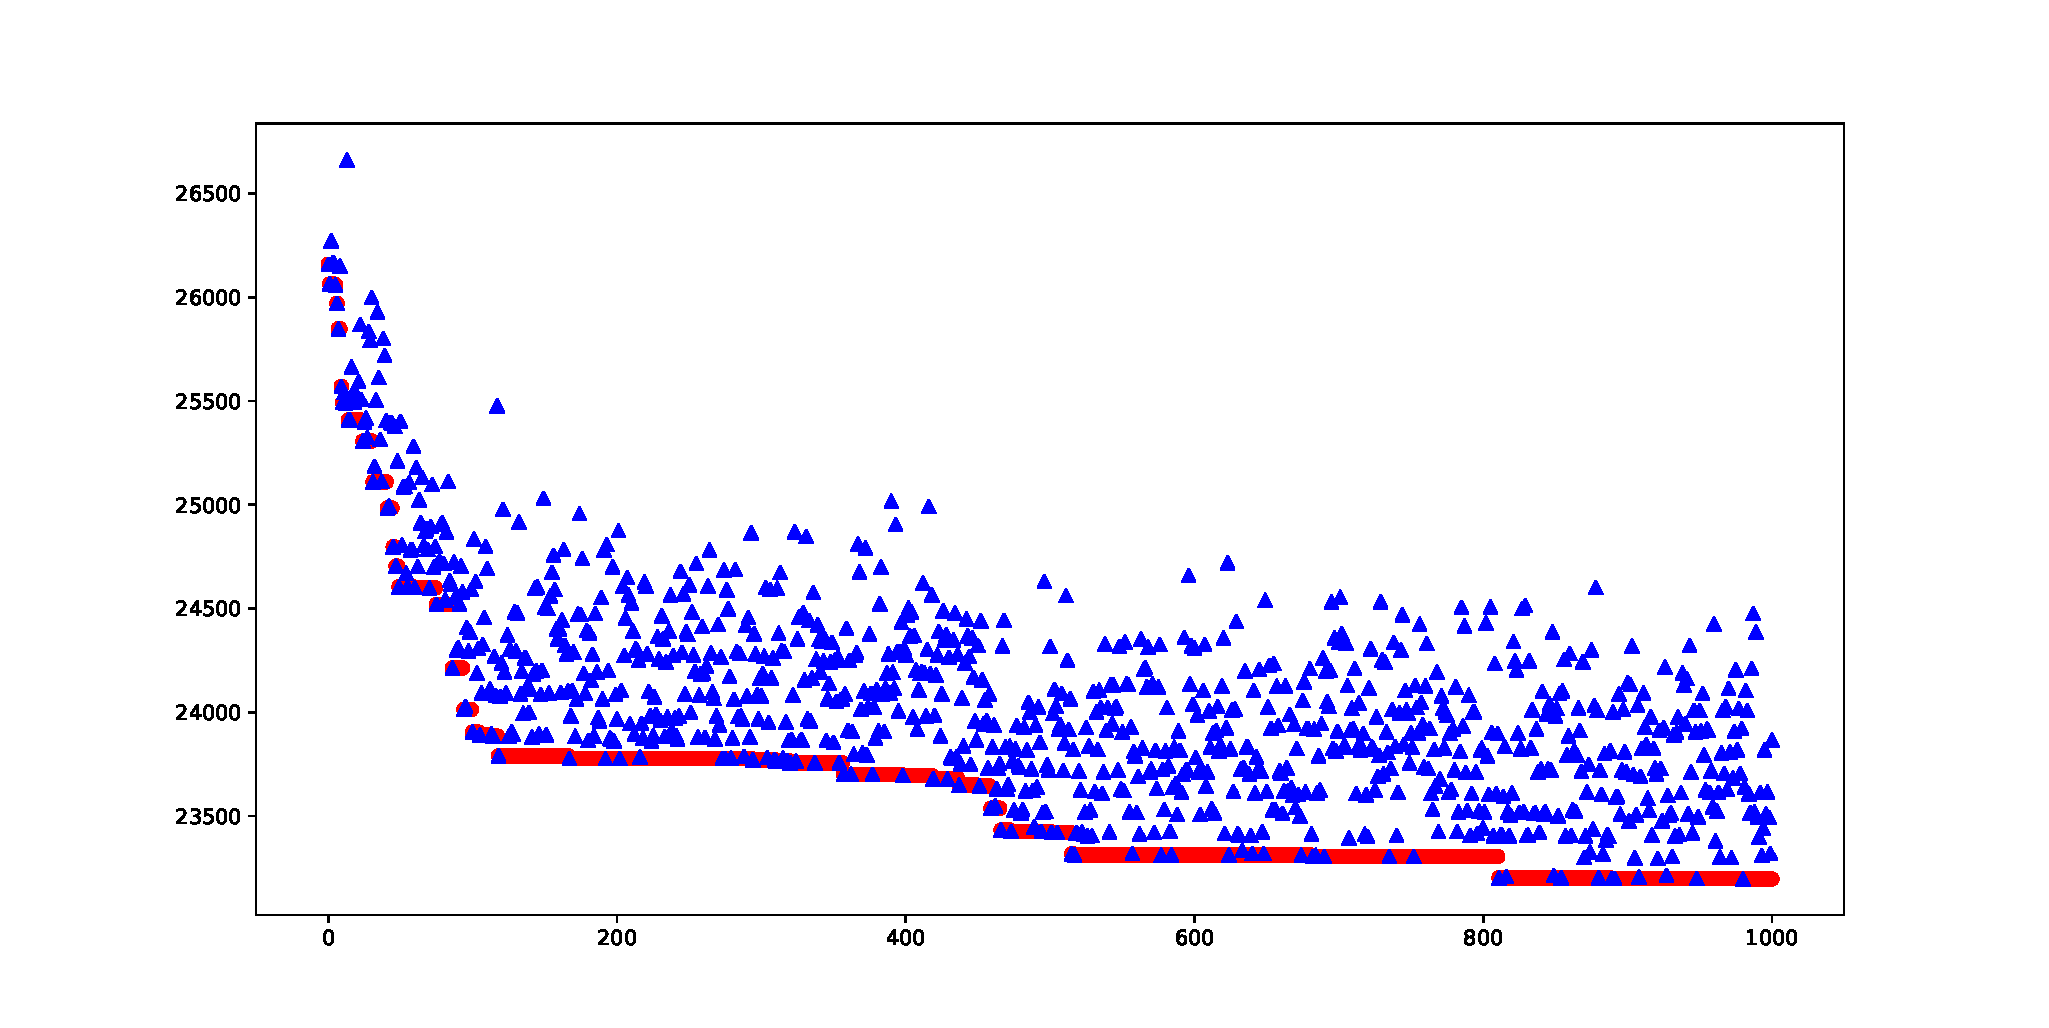
\includegraphics[scale=.4]{images/without_error_1000_v1}
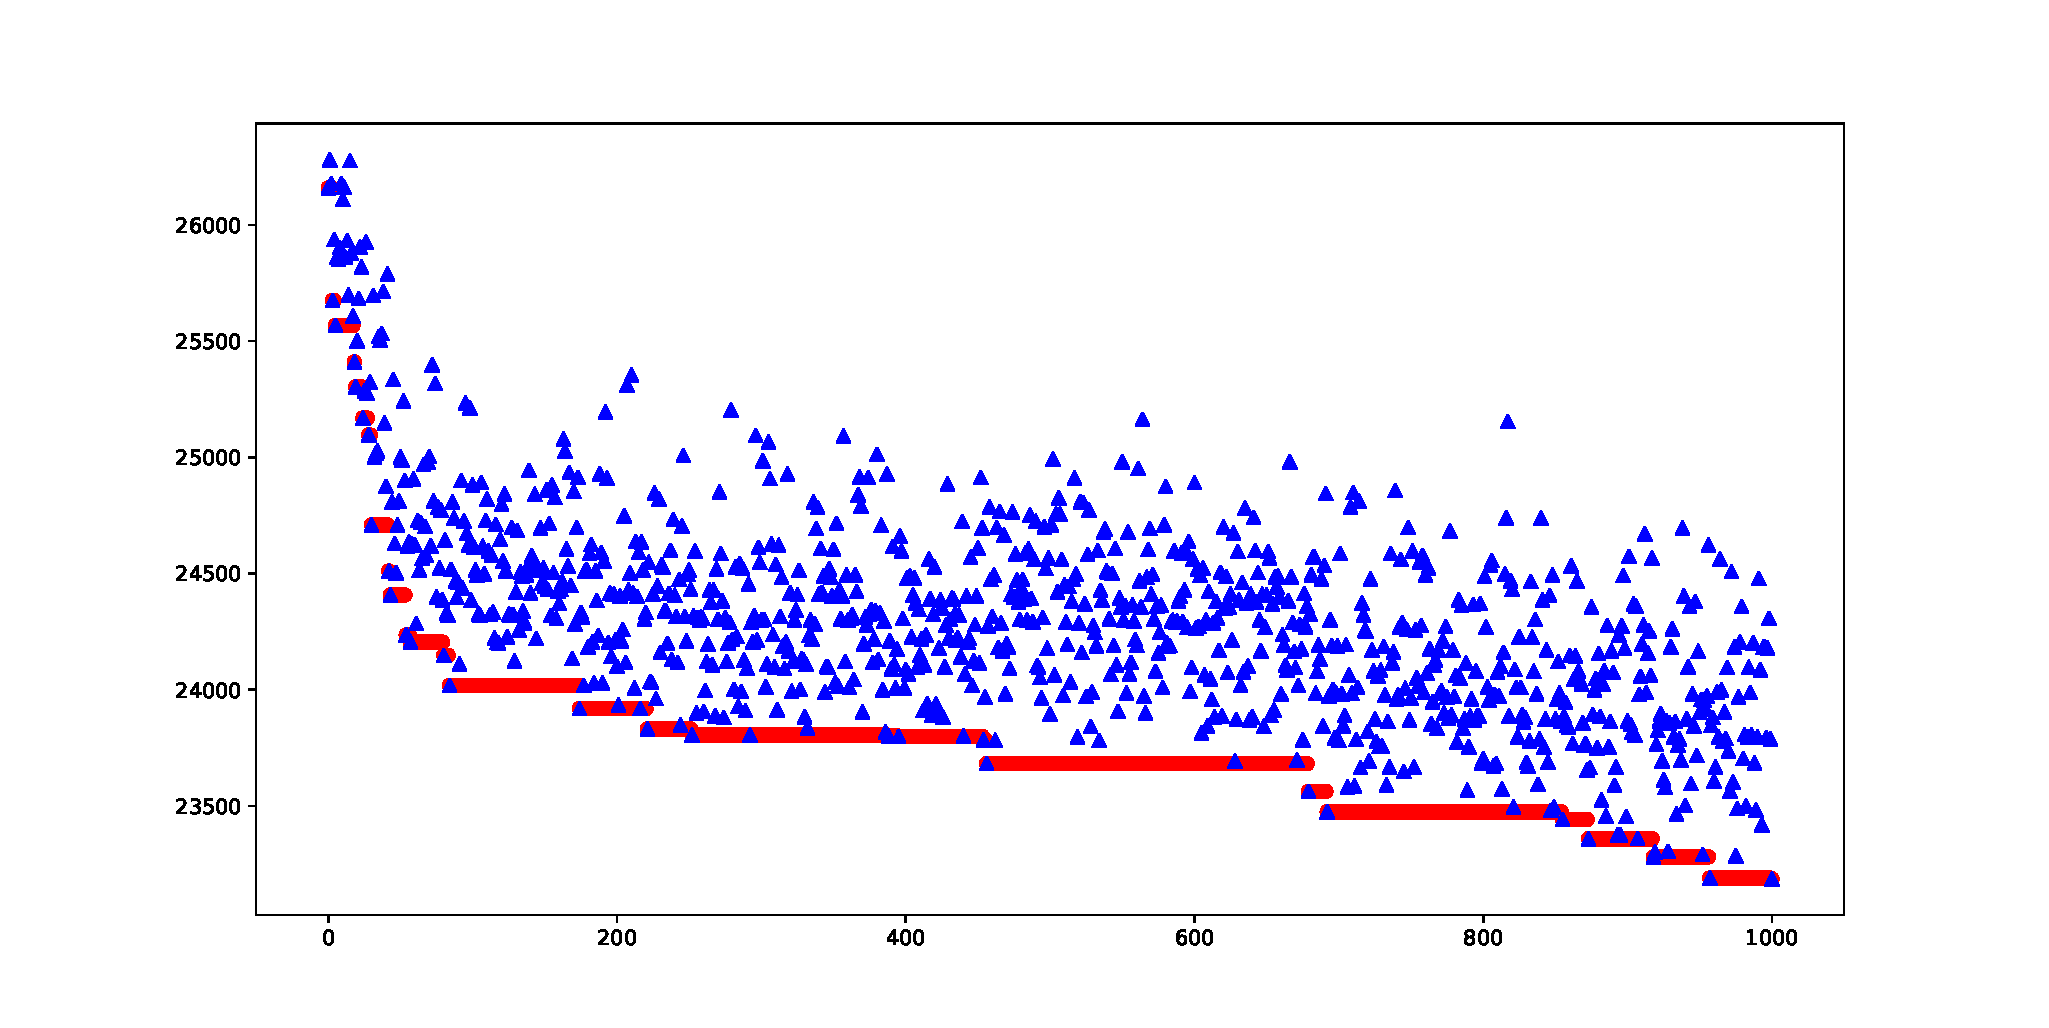
\includegraphics[scale=.4]{images/without_error_1000_v2}
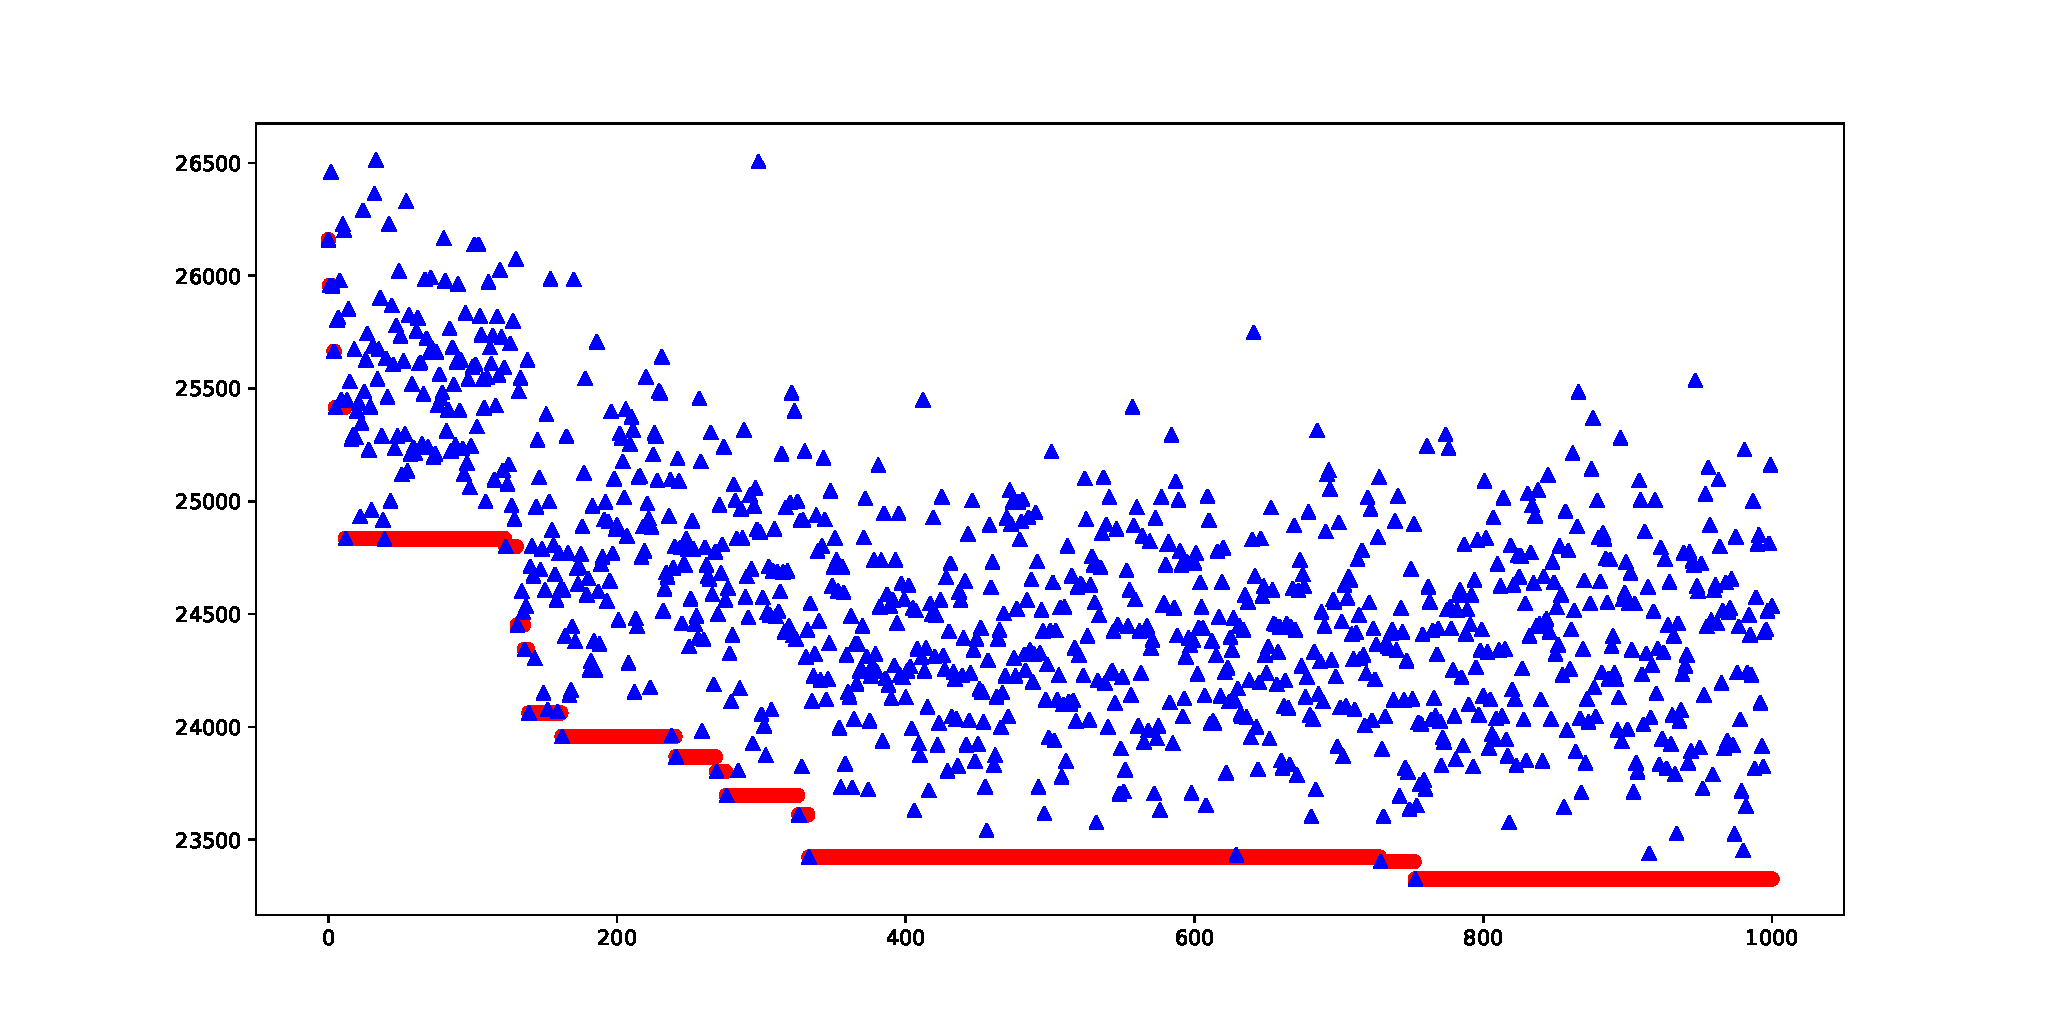
\includegraphics[scale=.4]{images/without_error_1000_v3}
\caption{Dans l'ordre de gauche à droite : version 1, 2, 3}
\end{figure}


\section{Local Searchs}

On va vouloir parcourir l'ensemble des solutions a la recherche de minimum locaux. Tout le problème de ces parcours est d'arriver a trouver de "bons" minimums locaux, il faut donc en général continuer a trouver un bon trade off entre l'exploration et l'exploitation des points visités.  

\subsection{Sans erreur}


Cf local\_search\_only\_better() dans le fichier simulated\_annealing.

Cette première version est la plus "simple". On n'explore pas du tout de nouvelles parties de notre espace de solution et on se contente de choisir de manière greedy la meilleure solution possible à chaque étape. Nous avons largement utilisé cette fonction pour comparer nos version de choix de voisins. 

\subsection{Avec erreur}

Cf local\_search\_with\_errors() dans le fichier simulated\_annealing.

Cette fois a chaque tour de boucle on s'autorise le choix d'une mauvaise solution. Ce choix est entièrement arbitraire et ne dépend pas de l'erreur que l'on va faire. On pourrait l'améliorer en choisissant une probabilité d'erreur dépendant de l'écart entre la solution actuelle  et de la solution que l'on va peut choisir.


\subsection{Recuit simulé}


\subsubsection{Présentation basique}

Le recuit simulé s'appuie sur ce principe de pouvoir choisir une mauvaise solution. Cependant la probabilité d'acceptation de la solution va être indexée sur deux paramètre : le delta entre les deux solutions, et les

\subsubsection{Choix de la température}


\section{Algorithmes biologiques}


\subsection{Algorithme moléculaire}


\subsubsection{Choix des }



\end{document}